% !TEX root =../main.tex
% Chapter 1

\chapter{Introduction} % Main chapter title

\label{Chapter1} % For referencing the chapter elsewhere, use \ref{Chapter1} 

%----------------------------------------------------------------------------------------

% Define some commands to keep the formatting separated from the content 
%\newcommand{\keyword}[1]{\textbf{#1}}
%\newcommand{\tabhead}[1]{\textbf{#1}}
%\newcommand{\code}[1]{\texttt{#1}}
%\newcommand{\file}[1]{\texttt{\bfseries#1}}
%\newcommand{\option}[1]{\texttt{\itshape#1}}

%----------------------------------------------------------------------------------------

\section{Calibration of a Gravitational-Wave detector}

KAGRA is a laser interferometer using four mirrors (test masses) suspended 
from multi-stage pendulums to form two perpendicular optical cavities (arms).
Gravitation Wave (GW) strain causes differential variations of the arm length
and generates power fluctuation in the detector readout port. 
The power fluctuations measured by photodetectors work as the GW readout 
signal and an error signal to control the differential arm length. 
For the stable operation of the instrument, a feedback control of the 
differential arm length is required. This control is achieved by taking 
a digitized readout signal, applying a set of digital filters, and sending 
the control signal to the test mass actuators. Therefore, estimation 
of the equivalent GW strain sensed by the interferometer requires 
detailed characterization and correction for the feedback control loop.

The calibration uncertainties are directly translated to the systematic 
errors on the absolute GW signal amplitude. In case of LIGO GW150914 event, 
the calibration was established to an uncertainty (1$\sigma$) of less than 
10\% in amplitude and 10 degrees in phase~\cite{GW150914}.
In case of LIGO GW151226 event, the calibration uncertainty (1$\sigma$) 
in both detectors at the time of the signal is better than 8\% 
in amplitude and 5 degrees in phase~\cite{GW151226}.

The primary impact of the calibration uncertainties to the physics parameters 
is the determination of the distance to the source. The 10\% uncertainties of 
the GW amplitude directly correspond to 10\% uncertainties on the estimation 
of the luminosity distance. Furthermore, since the estimation of the 
population of the GW sources depends on the third power of the source 
distance, 10\% calibration uncertainties will be translated into $\sim$30\% 
uncertainties on the population estimation.

The calibration uncertainties also affect the coordinate reconstruction 
particularly in the case that only up to three detectors in the world 
GW detector network can detect the GW signal. This can often happen 
because the sensitivity of interferometer has directional dependence. 
The effect of calibration uncertainties is visible at high signal-to-noise 
ratio events where the angular resolution is less affected by the detector 
noise. In such cases, the pointing accuracy can get worse by factor of 
2$\sim$4 with 10\% calibration uncertainties~\cite{Klimenko}.

%----------------------------------------------------------------------------------------

\newpage
\section{Roles of the photon calibrator}

Photon calibrators are the primary calibration tools in the Advanced LIGO 
and Advanced Virgo detectors~\cite{LIGO-CAL,Karki,Virgo-PCAL}.
Earlier versions have been tested on various 
interferometers~\cite{Accadia,Clubley:2001,Mossavi:2006},
and they have evolved significantly in LIGO over the past ten 
years~\cite{Goetz:2009}.
There are several unique roles required to the photon calibrator:

\begin{enumerate}
\item {\bf Check of the sign of \sl h(t)}\\
Since the direction of the movement of test mass is proportional to the 
laser power, photon calibrator allows a direct check of the sign of the 
reconstructed $h(t)$ channel compared to the definition taken in agreement 
with other experiments. In initial phase of Virgo, the primary purpose of 
photon calibrator was to check the sign of $h(t)$~\cite{VIR-018}.

\item {\bf Calibration during the observing periods}\\
Calibration methods without using photon calibrator such as using 
radio-frequency oscillator and laser wavelength can be done only under the 
limited condition where the interferometer is not operating in the optimum 
sensitivity. The propagation of calibration parameters from the high noise 
condition to the low noise condition can introduce additional unknown source 
of systematic errors. On the other hand, the photon calibrator is a completely 
independent instrument of the interferometer and therefore can actuate 
the test masses during the observation periods with optimum sensitivity. 

%\item {\bf Hardware injection}\\
%Hardware injection in the high frequency region is important to verify the 
%response of the detector system. Since actuators are inside the feedback 
%control loop, the amplitude is more suppressed for higher frequencies. 
%Photon calibrator can inject the high frequency signal more efficiently. 

\item {\bf Independence of calibration method\\
      and reliability assurance of interferometer}\\
Injecting calibration signals into the control feedback loop has a limitation 
to reduce the systematic errors because it is calibrating the loop itself.
Without Pcal, it is difficult to disentangle each uncertainty inside the loop, 
such as optical gain and actuator efficiency. On the other hand, Pcal has a 
strong advantage to enable to inject calibration signals independent of the 
control loop and provide an additional way to reduce the systematic 
uncertainties.

\item {\bf Globalization of the calibration}\\
It is necessary to calibrate and compare the absolute accuracies of KAGRA, 
LIGO and Virgo, or at least we need to have a way to evaluate the difference 
of absolute GW amplitude between different detectors. This kind of difference 
introduces bias on the physics parameters such as the source localization. 
Typical examples are cosmic-ray air shower observations and X-ray 
observations. In the long history of the air shower experiments, 
there have been always discussions about the absolute energy estimation. 
On the other hand, X-ray detector can be calibrated by the radio isotope 
sources and there is no question raised. In the GW experiment, absolute 
calibration is a difficult work but therefore it will be the key issue of the 
experimental verifications in the next decades.

\end{enumerate}


%----------------------------------------------------------------------------------------

\section{Schedule of KAGRA}

Fig.~\ref{fig:LVK} shows the 
In order to coincide the observation plan by LIGO and Virgo~\cite{LV-obs},
KAGRA is currently installing the instrument to meet the following observation
schedule~\cite{KAGRA-obs}:

\begin{enumerate}
\item Phase-1: 2017.3 -- 2018.3\\
      Operation of Michelson interferometer in cryogenic condition 
      followed by introducing Fabry P\'{e}rot cabity.
\item Phase-2: 2018.4 -- 2019.3 (Opening)\\
      Full lock of RSE (Resonant Sideband Extraction)
\item Phase-3: 2019.4 -- 2020.3 (Early) \\
      One year commissioning after the first full operation, 
      then improve the sensitivities to achieve the design goal
\item 2020 -- 2021: Middle term observation
\item 2021 -- 2022: Late term observation
\item 2022 -- : Observation with the designed sensitivity


\end{enumerate}
\begin{figure}
\begin{center}
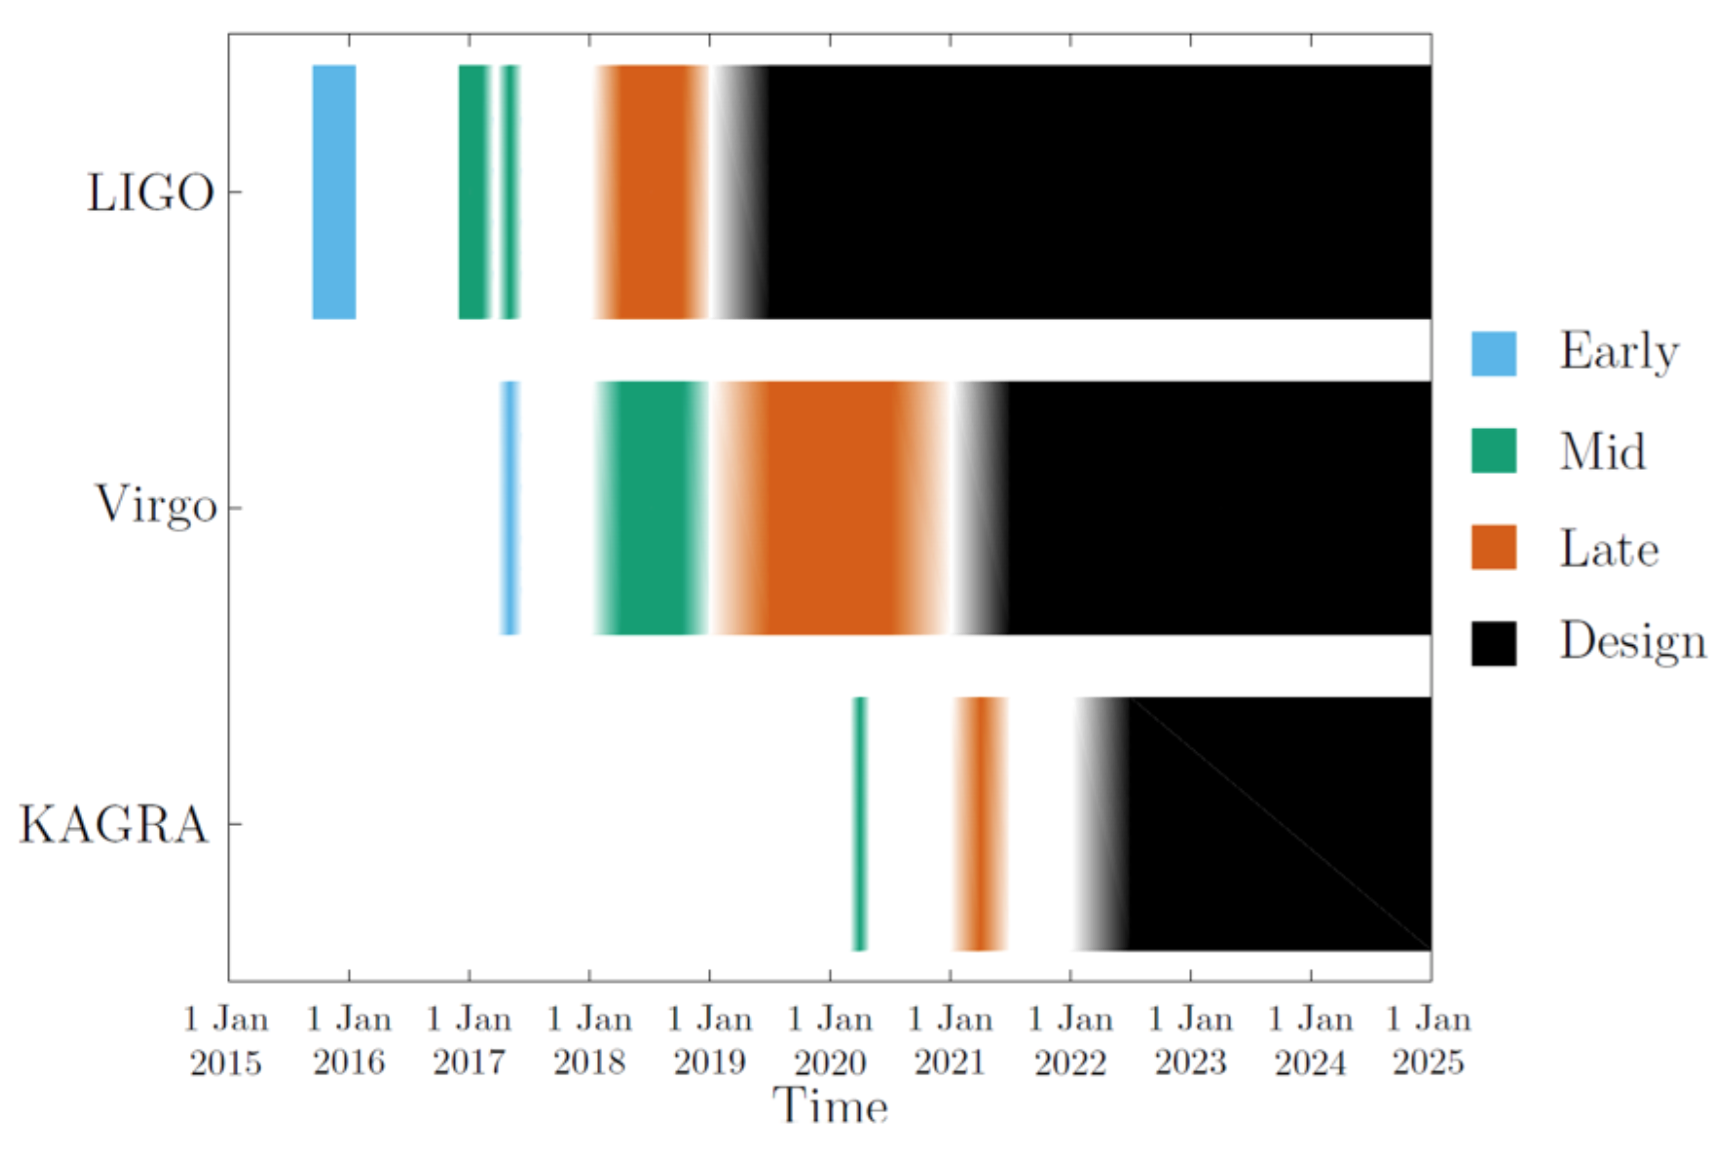
\includegraphics[width=15cm]{Figures/LVK.eps}
\caption{Observation scenario of LIGO, Virgo and KAGRA.} 
\label{fig:LVK} 
\end{center}
\end{figure}


%----------------------------------------------------------------------------------------

\section{Calibration requirements from data analysis}

A calibration accuracy will decide how precise scientific results can be extracted from various data 
analysis of gravitational wave events. We have to consider the error propagation not only from 
calibration accuracy to the reconstructed strain data both in time series $h(t)$ and frequency 
domain $h(f)$, but also from $h(t)$ and $h(f)$ to many cases of event analysis. However, parameter 
estimations in GW event data analysis now is not simple, e.g. employing Markov-chain Monte Carlo, 
Bayesian Estimation, higher-order waveforms, numerical simulated waveforms, etc. It is not so easy 
to conclude the requirement of the accuracy of calibration immediately. There are some challenges to 
estimate them in actual situation now. Here, we would like to introduce some typical cases of errors 
in event analysis. The calibration errors will be serious in high signal-to-noise ratio (S/N) 
events, but also effective on statistical estimation with many events.

One of the cases which can image the situation simply is parameter estimation of compact binary 
coalescence. If the 5\% amplitudes error of GW reflects as 5\% error on the distance estimation of 
the binary directly. For each event with low S/N (typically S/N$\sim$10), the errors are dominated by 
detector noises. However, when we discuss with 100 or more events, we may found the effects of 
calibration errors. For example, neutron stars/black-holes binary merger rate estimation may have 
15\% biases with 5\% biased $h(t)$. Or in cases of the events almost detection range (as like a few 
100 Mpc for neutron star binary, several 100~Mpc $\sim$ 1~Gpc for black-hole binary), 5\% distance 
errors will be comparable with the correction of cosmological redshift. If we would like to discuss 
the population of binaries, to do the geometrical test of universe expansion, the calibration 
accuracy be necessary as 1\% or less.

In the cases of multi-detector coincidence/coherence analysis are more serious on `absolute' 
calibration. When we compare the waveforms from a few detectors, the errors on the waveforms from 
each detector might make biases on the results. For example, the direction guess will be slightly 
sifted to the azimuthal direction of the detector which have larger amplitude. The inference of 
polarization and inclination angle may have biases. The propagation is complex, because the number of
parameters of compact binary stars are not small, at least nine without spin parameters. Similar 
biases will appear in stochastic GW analysis including radiometry.

Phase errors are also serious in multi-detector analysis. 
In compact binary case, phase errors of waveforms may cause errors on arrival time and mass of stars.
An arrival time error propagates immediately on an inference of the source direction.
Mass accuracy will reflect on the distance guess.
In case of burst waves, we need to analyze waveform coherence. It will make biases more seriously, because that the burst analysis has to treat the waveforms without 
certain analytic template waveforms by theory. It is well known that the phase error of the 
calibration will be large around the unity gain frequency, and such frequency is good sensitivity 
band in general. Therefore, it is very important to achieve the absolute calibration, that can be 
compared inter-observatories: LIGO, Virgo, KAGRA.

After the discovery of heavy black-hole binary GW150914, the science at the formation of larger 
black-hole after merging is attracting many people. Because, the black-hole physics will be possible 
at black-hole formation. Typical proposal is an analysis of the quasi-normal mode oscillation. When 
we extract the accurate waveform of ring-down gravitational waveform, it makes us possible to test 
the general relativity (GR). However, such accurate GR testing requires high S/N, because that the 
expected anomaly from GR is not so large. There is also another proposal of searching for `echo' 
waves from black-hole. In these cases, we need `gold-plated' events of high S/N larger than 30 or as 
like. These events are rare, however, approximately 2\% of events selected S/N>8 will have S/N >30, 
i.e. we may get a few events of S/N > 30 in whole of 100 events. 
In this high S/N events, the accuracy of calibration will be dominant factor of waveform study. 
We need high-fidelity of waveform for gold-plated events. 
Even such events are small numbers of, but these have impact on advanced feature of physics.

In the KAGRA observational era, we have to assume above situations : multiple detector observation, 
a few or several 100 events, and a few gold-plated events.


%----------------------------------------------------------------------------------------

